\chapter{Các công trình liên quan}
\label{chap:RelatedWork}

Trong phần này chúng tôi sẽ trình bày về các định nghĩa cơ bản về đồ thị tri thức, để từ đó hiểu được nhiệm vụ dự đoán liên kết trong đồ thị tri thức là gì cũng như các hướng nghiên cứu bên khác liên quan về đồ thị tri thức.

\section{Định nghĩa đồ thị tri thức}

Các định nghĩa cơ bản về đồ thị tri thức được nhóm tác giả Cai, Hongyun\cite{cai2018comprehensive} và Goyal, Palash\cite{goyal2018graph} tổng hợp và phân loại như sau :

\begin{figure}[htp]
	\centering
	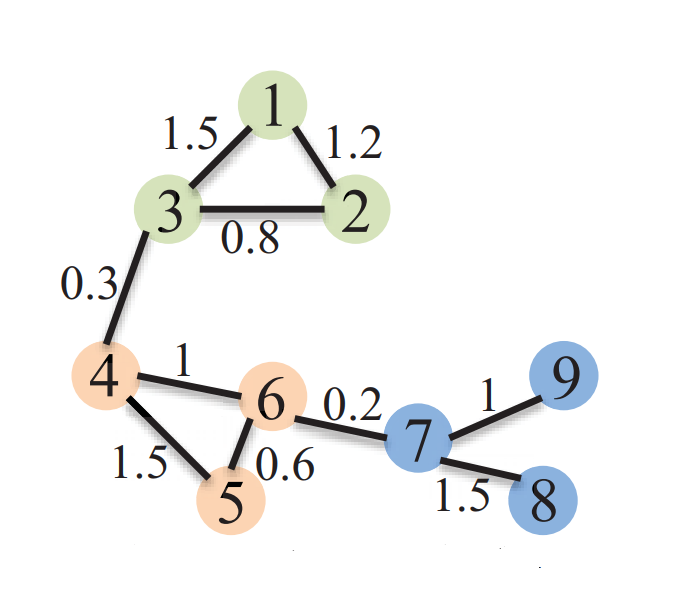
\includegraphics[width=7 cm]{images/graph_emb_1.png}
	\caption{Ví dụ về đồ thị đầu vào}
	\label{fig:graphInput}
\end{figure}

\begin{itemize}
	\item \begin{definition}[Đồ thị]\label{def:defGraph}
		\(\mathcal{G} = (V, E)\), trong đó \(v \in V\) là một đỉnh và \(e \in E\) là một cạnh. \(\mathcal{G}\) được liên kết với hàm ánh xạ loại đỉnh \(f_v: V \to T^v\) và hàm ánh xạ loại cạnh: \(f_e: E \to T^e\) .
	\end{definition}
	
	Trong đó: \(T^v\) và \(T^e\) lần lượt là tập hợp các loại đỉnh và loại cạnh. Mỗi đỉnh \(v_i \in V\) thuộc về một loại cụ thể, tức là, \(f_v(v_i) \in T^v\). Tương tự, đối với \(e_{ij} \in E, f_e (e_{ij}) \in T^e\).
	
	\item
	\begin{definition}[Đồ thị đồng nhất]\label{def:homogeneous}
		Đồ thị đồng nhất (homogeneous graph) : \textit{ $\mathcal{G}_{homo} = (V, E)$ là đồ thị trong đó $\mid T^v \mid = \mid T^e \mid = 1$. Tất cả các đỉnh trong $\mathcal{G}$ thuộc về một loại duy nhất và tất cả các cạnh thuộc về một loại duy nhất}.
	\end{definition}
	
	\item
	\begin{definition}[Đồ thị không đồng nhất]\label{def:heterogeneous}
		Đồ thị không đồng nhất (heterogeneous graph) : \textit{$\mathcal{G}_{hete} = (V, E)$ là một đồ thị trong đó $\mid T^v \mid > 1$ hoặc $\mid T^e \mid > 1$. Tức là có nhiều hơn một loại đỉnh hoặc nhiều hơn một loại cạnh}.
	\end{definition}
	
	\item
	\begin{definition}[Đồ thị tri thức]\label{def:knowledgeGraph}
		Đồ thị tri thức (knowledge graph)
		$\mathcal{G}_{know} = (V, R, E)$ là một đồ thị có hướng, có tập đỉnh là biểu diễn cho các thực thể (entities), tập quan hệ biểu diễn các mối quan hệ (relations) giữa các đỉnh, tập cạnh (edges) biểu diễn các sự kiện $E \subseteq V\times R \times V$ là gồm bộ ba subject-property-object. Mỗi cạnh là một mẫu gồm $(\text{entity}_{\text{head}}, \text{relation}, \text{entity}_{\text{tail}})$ (ký hiệu là $\langle h, r, t \rangle$) biểu thị mối quan hệ của $r$ từ thực thể $h$ đến thực thể $t$ .
	\end{definition}
	Trong đó $h, t \in V$ là các thực thể và $r \in R$ là các quan hệ. Chúng ta gọi $\langle h, r, t \rangle$ một bộ ba (triples) đồ thị tri thức.
	
	Ví dụ: trong hình \ref{fig:graphExample} có hai bộ ba: $\langle \text{Tom\ Cruise,\ born_in,\ New\ York} \rangle$ và $\langle \text{New York, state_of, U.S} \rangle$. Lưu ý rằng các thực thể và quan hệ trong đồ thị tri thức thường có các loại khác nhau. Do đó, đồ thị tri thức có thể được xem như là một ví dụ của đồ thị không đồng nhất.
\end{itemize}

\section{Dự đoán liên kết trong đồ thị tri thức}

Dự đoán liên kết (link prediction) hay hoàn thiện đồ thị tri thức (knowledge graph completion) là nhiệm vụ khai thác những sự kiện có sẵn trong đồ thị tri thức để suy luận ra sự kiện còn thiếu. Điều này tương đương với việc đoán đúng thực thể đuôi $\langle h, r, ? \rangle$ (dự đoán đuôi) hoặc $\langle ?, r, t \rangle$ (dự đoán đầu). Để đơn giản,  thay vì gọi dự đoán đầu hoặc đuôi, một cách tổng quát chúng ta gọi thực thể nguồn (source) là thực thể đã biết trong việc dự đoán, thực thể đích (target) là cái chúng ta cần dự đoán.


Hầu hết các nghiên cứu hiện tại về việc dự đoán liên kết của đồ thị tri thức đều liên quan đến các phương pháp tiếp cận tập trung vào khái niệm nhúng một đồ thị đã cho trong một không gian vectơ có số chiều thấp. Ngược lại với các tiếp cận này là một phương pháp đựa trên luật được nghiên cứu trong \cite{burl}. Thuật toán cốt lõi của nó dựa trên lấy mẫu một luật bất kỳ, sau đó khái quát  thành các quy tắc Horn\cite{wiki:Horn}. Tiếp đó dùng thống kê để tính độ tin cậy của các luật được khái quát. Khi dự đoán một liên kết mới (cạnh mới) của đồ thị chúng ta dự đoán một đỉnh có cạnh nối với một quan hệ cụ thể (label) với đỉnh còn lại hay không. Cũng đã có rất nhiều phương pháp được nghiên cứu, đề xuất để học các các luật trong đồ thị chẳng hạn như trong  RuDiK\cite{ortona2018robust}, AMIE\cite{galarraga2015fast}, RuleN\cite{meilicke2018fine}. 
Như đã nói trong phần trước có hai cách tiếp cận chính cho bài toán này một là tối ưu hóa hàm mục tiêu. Tìm ra một bộ quy tắc nhỏ bao gồm phần lớn các ví dụ là đúng và ít sai sót nhất có thể như được ngiên cứu trong RuDiK\cite{ortona2018robust}. Còn cách tiếp cận còn lại cũng là cách tiếp cận mà chúng tôi chọn nghiên cứu là cố gắng tìm hiểu mọi quy tắc khả thi có thể sau đó tạo xếp hạng \(k\) ứng viên tiềm năng với một độ tin cậy nhất định được đo trên tập huấn luyện.

Phương pháp đựa trên luật của chúng tôi phần lớn dựa vào phương pháp Anytime Bottom-Up Rule Learning for Knowledge Graph Completion \cite{meilicke2019anytime} mà sau đây chúng tôi gọi là \textbf{AnyBURL}. Như tên của phương pháp này phương pháp chủ yếu chú trọng vào vấn đề hoàn thành đồ thị, điền những phần còn thiếu vào đồ thị. Vấn đề tồn đọng lại ở mô hình này khi có một cạnh mới hay một tri thức mới được thêm vào đồ thị sẽ phải đào tạo lại toàn bộ mô hình. Chúng tôi giải quyết vẫn đề này theo hai chiến lược offline-to-online tức là khi thêm vào đồ thị tập hợp các cạnh thì mới thực hiện lại quá trình đào tạo lại một phần của đồ thị và chiến lược thứ 2 là online-to-online  khi thêm một cạnh mới sẽ thực hiện đào tạo lại ngay một phần có liên quan tới cạnh vừa thêm vào.

% GAT
Trong nhánh các phương pháp về học sâu, rất nhiều kỹ thuật học sâu thành công trong xử lý ảnh và xử lý ngôn ngữ tự nhiên được áp dụng vào đồ thị tri thức như : Mạng Neural Tích Chập (Convolution Neural Network - CNN \cite{lecun1999object}), Mạng Neural Hồi Quy (Recurrent Neural Network\cite{hopfield2007hopfield}), và gần đây như Transformer (\cite{yang2019xlnet}), Mạng Neural Bao Bọc (Capsule Neural Network - CapsNet \cite{sabour2017dynamic}). Bên cạnh đó các nghiên cứu còn sử dụng một số kỹ thuật khác như Random Walks, các mô hình dựa trên cấu trúc phân cấp, .. Ưu điểm chung của nhóm các phương pháp học sâu trên đồ thị tri thức đó là tự động rút trích các đặc trưng và có thể khái quát hóa cấu trúc phức tạp của đồ thị dựa trên một lượng lớn dữ liệu huấn luyện. Tuy nhiên, một số phương pháp chỉ chủ yếu tập trung vào cấu trúc dạng lưới mà không giữ được đặc trưng không gian của đồ thị tri thức. 
Cơ chế chú ý hay lớp chú ý đa đỉnh (multi-head attention layer) đã được áp dụng vào đồ thị bằng mô hình Mạng Đồ Thị Chú Ý (Graph Attention Network - GAT \cite{velivckovic2017graph}) giúp tổng hợp thông tin của một thực thể dựa vào trọng số chú ý của thực thể gốc đối với các thực thể lân cận. Tuy nhiên, mô hình đồ thị chú ý lại thiếu thông tin của vector nhúng quan hệ cũng như các vector nhúng lân cận của một thực thể gốc, một phần rất quan trọng giúp thể hiện vai trò của từng thực thể. Vấn đề đó đã được giải quyết trong báo cáo Learning Attention-based Embeddings for Relation Prediction in
Knowledge Graphs (\textbf{KBAT} \cite{nathani2019learning}), mô hình được chúng tôi chọn làm cơ sở nghiên cứu.
Cơ chế chú ý đang là một trong những cấu trúc học sâu đạt được hiệu quả nhất hiện nay (state-of-the-art) vì nó đã được chứng minh là thay thế cho bất kỳ phương pháp tính tích chập nào \cite{cordonnier2019relationship},
hơn nữa nó cũng nằm trong cấu trúc cơ bản để áp dụng trên các mô hình mới nhất trên ngôn ngữ tự nhiên như mô hình Megatron-LM \cite{shoeybi2019megatron}, và trên phân đoạn hình ảnh như mô hình HRNet-OCR (Hierarchical Multi-Scale Attention \cite{tao2020hierarchical}). Một số phương pháp thú vị \cite{cordonnier2020multi} đã cải tiến dựa trên cơ chế chú ý, tuy nhiên nó lại chưa được áp dụng vào đồ thị tri thức, vì vậy chúng tôi chọn nhóm phương pháp này để áp dụng các cải tiến mới nhất vào đồ thị tri thức.

\section{Các lĩnh vực nghiên cứu về đồ thị tri thức}

\begin{figure}[htp]
	\centering
	\tikzset{
		category/.style  = {draw, font=\sffamily, thin, align=center},
		subcat/.style={rectangle, rounded corners=6pt},
		center/.style = {category, ellipse, fill=blue!60, text width=4em},
		group/.style = {category, subcat, fill=blue!30, rounded corners=6pt, text width=6em},
		yellowbox/.style = {category, subcat, fill=yellow!30},
		greenbox/.style = {category, subcat, fill=green!30},
		redbox/.style = {category, subcat, fill=red!30},
		bluebox/.style = {category, subcat, fill=cyan!30},
		leafbox/.style = {category, subcat, fill=black!10, rounded corners=0mm}
	}
	\resizebox{\textwidth}{!}{%
		\begin{tikzpicture}
			\node[center] (root) {Đồ thị tri thức};
			\node[group][above left=1cm of root] (c1) {Học biểu diễn tri thức};
			\node[group][above right=8mm of root] (c2) {Nhận biết tri thức};
			\node[group][below left=5mm of root] (c3) {Thu nhận tri thức};
			\node[group][below right=20mm of root, xshift=-2cm] (c4) {Đồ thị tri thức thời gian};
			
			\begin{scope}[every node/.style={yellowbox}]
				\node[above=8mm of c1, xshift=-1cm] (c11) {Biểu diễn không gian};
				\node[left=of c1, yshift=9mm, xshift=-10mm] (c12) {Hàm đánh giá};
				\node[left=15mm of c1, yshift=-5mm] (c13) {Mã hóa mô hình};
				\node[left=of c1, yshift=-20mm] (c14) {Thông tin tương tự};
			\end{scope}
			
			\begin{scope}[every node/.style={redbox}]
				\node[above left=of c2, text width=35mm, yshift=1mm, xshift=18mm] (c21) {Hiểu ngôn ngữ tự nhiên};
				\node[above=1cm of c2, yshift=5mm, xshift=13mm] (c22) {Trả lời câu hỏi};
				\node[right=of c2, yshift=15mm] (c23) {Hệ thống hội thoại};
				\node[right=of c2, yshift=-2mm] (c24) {Hệ thống gợi ý};
				\node[below=5mm of c2, xshift=5mm] (c25) {Ứng dụng khác};
			\end{scope}
			
			\begin{scope}[every node/.style={greenbox}]
				\node[left=1cm of c3, yshift=5mm] (c31) {Khai phá thực thể};
				\node[below left=of c3, yshift=1cm, xshift=3mm] (c32) {Rút trích quan hệ};
				\node[below right=5mm of c3, xshift=-4cm] (c33) {Hoàn thiện đồ thị};
			\end{scope}
			
			\begin{scope}[every node/.style={bluebox}]
				\node[below=of c4, xshift=-15mm, yshift=-35mm] (c41) {Lý giải logic thời gian};
				\node[below=of c4, xshift=2cm, yshift=-23mm] (c42) {Quan hệ thời gian độc lập};
				\node[below right=of c4,xshift=-2mm, yshift=-10mm] (c43) {Thực thể động};
				\node[right=of c4, yshift=-2cm, xshift=15mm] (c44) {Nhúng thời gian};
			\end{scope}
			
			\begin{scope}[every node/.style={leafbox}]
				\node[above=5mm of c11] (c11x) {
					\begin{tabular}{@{}l@{}@{}l@{}}
						-Point-wise & -Đa tạp \\
						-Số phức & -Gausian \\
						-Rời rạc & \\
					\end{tabular}
				};
				\node[above=5mm of c12, xshift=-5mm] (c12x) {
					\begin{tabular}{@{}l@{}}
						-Khoảng cách \\
						-Ngữ nghĩa \\
						-Khác \\
					\end{tabular}
				};
				\node[left=of c13, yshift=5mm] (c13x) {
					\begin{tabular}{@{}l@{}}
						-Tuyến tính/ \\song tuyến tính \\
						-Ma trận hóa \\
						-Neural Nets \\
						-CNN \\
						-RNN \\
						-Transformers \\
						-GCN \\
					\end{tabular}
				};
				\node[below left=5mm of c14, xshift=6mm, yshift=-7mm] (c14x) {
					\begin{tabular}{@{}l@{}c@{}l@{}}
						-Văn bản & -Kiểu & -Trực quan \\
					\end{tabular}
				};
				%%%%%%%%%%%% 
				\node[below left=of c31] (c31x) {
					\begin{tabular}{@{}l@{}}
						-Nhận dạng \\
						-Định kiểu \\
						-Phân biệt \\
						-Sắp xếp \\
					\end{tabular}
				};
				\node[below=of c32, xshift=-5mm] (c32x) {
					\begin{tabular}{@{}l@{}}
						-Neural Nets\\
						-Chú ý \\
						-GCN \\
						-GAN \\
						-RL \\
						-Khác \\
					\end{tabular}
				};
				\node[below=5mm of c33] (c33x) {
					\begin{tabular}{@{}l@{}}
						-Nhúng dựa trên xếp hạng\\
						-Lý giải đựa trên đoạn \\
						-Lý giải dựa trên luật \\
						-Học siêu quan hệ \\
						-Phân loại bộ ba \\
					\end{tabular}
				};
				%%%%%%%%%%%%%%%%%
				\node[above=5mm of c22] (c22x) {
					\begin{tabular}{@{}l@{}}
						-Single-fact QA\\
						-Lý giải nhiều bước \\
					\end{tabular}
				};
				\node[below right=5mm of c25, yshift=15mm] (c25x) {
					\begin{tabular}{@{}l@{}}
						-Sinh câu hỏi\\
						-Công cụ tìm kiếm \\
						-Ứng dụng y khoa \\
						-Hồi phục sức khỏe \\
						-Phân loại ảnh zero-shot\\
						-Sinh văn bản\\
						-Phân tích ngữ nghĩa\\
					\end{tabular}
				};
				
			\end{scope}
			
			\foreach \value in {1,...,4}
			\draw[->, line width=0.8mm] (root) -> (c\value);
			
			\foreach \value in {1,...,4}
			\draw[->, ultra thick] (c1) -> (c1\value);
			\foreach \value in {1,...,4}
			\draw[->, thick] (c1\value) -> (c1\value x);
			
			\foreach \value in {1,...,5}
			\draw[->, ultra thick] (c2) -> (c2\value);
			\foreach \value in {2,5}
			\draw[->, thick] (c2\value) -> (c2\value x);
			
			\foreach \value in {1,...,3}
			\draw[->, ultra thick] (c3) -> (c3\value);
			\foreach \value in {1,...,3}
			\draw[->, ultra thick] (c3\value) -> (c3\value x);
			
			\foreach \value in {1,...,4}
			\draw[->, ultra thick] (c4) -> (c4\value);
			
	\end{tikzpicture}}
	\caption{
		Danh mục các lĩnh vực nghiên cứu trên đồ thị tri thức}
	\label{fig:categoriesResearch}
\end{figure}

Biểu diễn tri thức đã từng có lịch sử phát triển suốt chiều dài lịch sử trong lĩnh vực logic và trí tuệ nhân tạo. Trên đồ thị tri thức, có 4 bốn nhóm nghiên cứu chính đã được phân loại và tổng hợp ở báo cáo \cite{ji2020survey} bao gồm : Học Biểu Diễn Tri Thức (Knowledge Representation Learning), Thu Nhận Tri Thức (Knowledge Acquisition), Đồ Thị Tri Thức Về Thời Gian (Temporal Knowledge Graphs), Ứng Dụng Nhận Biết Tri Thức (Knowledge-aware Applications). Tất cả các danh mục nghiên cứu được minh họa ở hình \ref{fig:categoriesResearch}.

\textbf{Học biểu diễn tri thức}

Học biểu diễn tri thức là vấn đề tìm hiểu thiết yếu của đồ thị tri thức giúp mở ra rất nhiều ứng dụng trong thực tế. Học biểu diễn tri thức được phân loại thành bốn nhóm con bao gồm : 

\begin{itemize}
	\item \textit{Biểu Diễn Không Gian} (Representation Space) nghiên cứu về cách các thực thể và quan hệ được biểu diễn trong không gian. Biểu diễn không gian bao gồm không gian điểm (point-wise), đa tạp (manifold), không gian vector số phức (complex), phân phối Gaussian và không gian rời rạc.
	
	\item \textit{Hàm Đánh Giá} (Scoring Function) nghiên cứu về hàm đo lường giá trị của một bộ ba trong thực tế, bao gồm các hàm đánh giá dựa trên khoảng cách hoặc dựa trên sự tương đồng.
	
	\item \textit{Mã Hóa Mô Hình} (Encoding Models) nghiên cứu về cách biểu diễn và học các tương tác giữa các mối quan hệ. Đây là hướng nghiên cứu chính hiện nay, bao gồm các mô hình tuyến tính hoặc phi tuyến tính, phân rã ma trận hoặc mạng neural.
	
	\item \textit{Thông Tin Bổ Trợ} (Auxiliary Information) nghiên cứu về cách kết hợp vào các phương pháp nhúng, các thông tin bổ trợ bao gồm văn bản, hình ảnh và loại thông tin .
\end{itemize}

\textbf{Thu nhận tri thức}

Thu nhận tri thức nghiên cứu về cách thu nhận tri thức dựa trên đồ thị tri thức, bao gồm hoàn thiện đồ thị (knowledge graph completion), khai thác quan hệ và khai phá thực thể. Khai thác quan hệ và khai phát thực thể là nhóm phương pháp khai thác tri thức mới (bao gồm các quan hệ hoặc thực thể) trong đồ thị từ văn bản. Hoàn thiện đồ thị là nhiệm vụ mở rộng đồ thị tri thức dựa trên đồ thị đang có. Hoàn thiện đồ thị bao gồm các hướng nghiên cứu như : xếp hạng dựa trên nhúng (embedding-based ranking), dự đoán đường đi quan hệ (relation path reasoning), dự đoán dựa trên luật (rule-based reasoning) và học siêu quan hệ.
Khai phá thực thể bao gồm nhận dạng, phân biệt, định kiểu và sắp xếp. 
Các mô hình khai thác quan hệ sử dụng cơ chế chú ý, mạng đồ thị tích chập (graph
convolutional networks), huấn luyện đối nghịch (adversarial training), học tăng cường (reinforcement learning), học sâu và học chuyển tiến (transfer learning), đây là hướng nghiên cứu trong phương pháp đề xuất của chúng tôi.

Ngoài ra, trên đồ thị tri thức còn có các hướng nghiên cứu như \textbf{đồ thị tri thức về thời gian} và \textbf{ứng dụng nhận biết tri thức}. Đồ thị tri thức về thời gian sẽ kết hợp thêm thông tin thời gian trên đồ thị để học cách biểu diễn, còn ứng dụng nhận biết tri thức bao gồm hiểu ngôn ngữ tự nhiên (natural language understanding), trả lời câu hỏi (question answering), hệ thống gợi ý (recommendation systems) và nhiều nhiệm vụ khác trong thế giới thực mà nó tích hợp tri thức vào để cải thiện quá trình học biểu diễn .